\selectlanguage{english}%

\chapter{Modelagem}
\label{capMod}
Os modelos físicos do sistema de quatro-tanques utilizados neste trabalho são apresentados nas seções a seguir.

\section{Modelo Não Linear}
Baseado nos princípios de conservação de massa e na lei de Bernoulli para líquidos incompressíveis tem-se o seguinte sistema de equações não lineares que descrevem o processo.

\begin{equation} \label{eqModNL}
	\begin{cases}
		\dot{h_{1}} = \frac{1}{A_{1}}(a_{3}\sqrt{2gh_{3}} + \gamma_{1}k_{1}v_{1} - a_{1}\sqrt{2gh_{1}})\\
		
		\dot{h_{2}} = \frac{1}{A_{2}}(a_{4}\sqrt{2gh_{4}} + \gamma_{2}k_{2}v_{2} - a_{2}\sqrt{2gh_{2}})\\
		
		\dot{h_{3}} = \frac{1}{A_{3}}((1 - \gamma_{2})k_{2}v_{2} - a_{3}\sqrt{2gh_{3}})\\
		
		\dot{h_{4}} = \frac{1}{A_{4}}((1 - \gamma_{1})k_{1}v_{1} - a_{4}\sqrt{2gh_{4}})
	\end{cases}
\end{equation}

Na \jhhref{eqModNL}{Equação}, os termos $h_{i}$, $A_{i}$ e $a_{i}$ representam o nível de água, a área da secção transversal da base do tanque $i$ e a área de secção transversal do orifício de saída do tanque $i$, $i=1,2,3,4$, respectivamente. A constante de fluxo da bomba $j$ e a tensão aplicada sobre ela são dadas por $k_{j}$ e $v_{j}$, $j=1,2$. O parâmetro $\gamma_{1}$ é a razão entre os fluxos para os tanques 1 e 4 enquanto $\gamma_{2}$ é a razão entre os fluxos para os tanques 2 e 3 e g é a aceleração da gravidade. 

É fácil notar nas equações deste sistema os termos não lineares (as raízes). O aspecto do acoplamento entre as variáveis também pode ser observado ao analisar as equações: o nível $h_1$ varia conforme o fluxo da bomba 1, dependente de $v_1$, e conforme o nível $h_3$, que por sua vez depende do fluxo da bomba 2, $v_2$. Assim, as variáveis manipuladas, $v_1$ e $v_2$, influem em ambos os níveis simultaneamente, apresentando um desafio considerável para a estabilização dos níveis desejados, $h_1$ e $h_2$, que são as variáveis controladas deste trabalho.

\section{Linearização}
Linearizando o sistema em torno dos ponto de operação $\overline{h}=(\overline{h_{1}},\overline{h_{2}},\overline{h_{3}},\overline{h_{4}})$ e $\overline{v}=(\overline{v_{1}},\overline{v_{2}})$, por expansão em série de Taylor, obtém-se a seguinte representação no espaço de estados:

\begin{multline} \label{eqModLinear}
	\begin{bmatrix}
		\dot{\Delta h_{1}} \\
		\dot{\Delta h_{2}} \\
		\dot{\Delta h_{3}} \\
		\dot{\Delta h_{4}} 
	\end{bmatrix}
	= 
	\begin{bmatrix}
		\frac{-a_{1}\sqrt{2g}}{2A_{1}\sqrt{h_{1}}} & 0 & \frac{a_{3}\sqrt{2g}}{2A_{1}\sqrt{h_{3}}} & 0 \\
		0 & \frac{-a_{2}\sqrt{2g}}{2A_{2}\sqrt{h_{2}}} & 0 & \frac{a_{4}\sqrt{2g}}{2A_{2}\sqrt{h_{4}}} \\
		0 & 0 & \frac{-a_{3}\sqrt{2g}}{2A_{3}\sqrt{h_{3}}} & 0 \\
		0 & 0 & 0 & \frac{-a_{4}\sqrt{2g}}{2A_{4}\sqrt{h_{4}}}
	\end{bmatrix}
	\begin{bmatrix}
		\Delta h_{1} \\
		\Delta h_{2} \\
		\Delta h_{3} \\
		\Delta h_{4} 
	\end{bmatrix}
	+
	\begin{bmatrix}
		\frac{\gamma_{1}k_{1}}{A_{1}} & 0 \\
		0 & \frac{\gamma_{2}k_{2}}{A_{2}} \\
		0 & \frac{(1-\gamma_{2}) k_{2}}{A_{3}} \\
		\frac{(1-\gamma_{1})k_{1}}{A_{4}} & 0
	\end{bmatrix}
	\begin{bmatrix}
		\Delta v_{1} \\
		\Delta v_{2}
	\end{bmatrix}
\end{multline}
\begin{equation}
	\begin{bmatrix}
		y_{1} \\
		y_{2} \\
		y_{3} \\
		y_{4} 
	\end{bmatrix}
	= 
	I
	\begin{bmatrix}
		\Delta h_{1} \\
		\Delta h_{2} \\
		\Delta h_{3} \\
		\Delta h_{4} 
	\end{bmatrix}
	\label{eq3}
\end{equation}

em que $y_{i}$ são as saídas medidas do sistema, $\Delta h_{i}=h_{i} - \overline{h_{i}}$, $\Delta v_{i}=v_{i} - \overline{v_{i}}$, e $i=1,2,3,4$.

E por fim, a matriz função de transferência do sistema obtida é:
\begin{equation}
		G(s) = 
	\begin{bmatrix}
		\frac{T_{1}\gamma_{1}k_{1}}{A_{1}(1+sT_{1})} &  \frac{T_{1}(1-\gamma_{2})k_{2}}{A_{1}(1+sT_{3})(1+sT_{1})} \\
		\frac{T_{2}(1-\gamma_{1})k_{1}}{A_{2}(1+sT_{4})(1+sT_{2})} &  \frac{T_{2}\gamma_{2}k_{2}}{A_{2}(1+sT_{2})} \\
		0 &  \frac{T_{3}(1-\gamma_{2})k_{2}}{A_{3}(1+sT_{3})} \\
		\frac{T_{4}(1-\gamma_{1})k_{1}}{A_{4}(1+sT_{4})} &  0 
	\end{bmatrix} 
	\label{eq4}
\end{equation}

em que $G(s)=\frac{\Delta h(s)}{\Delta v(s)}$ e $T_{i}=\frac{2A_{i}\sqrt{h_{i}}}{a_{i}\sqrt{2g}}$, $i=1,2,3,4$.

\section{Modelagem Fuzzy Takagi-Sugeno} \label{secModFuzzy}
A modelagem via Takagi-Sugeno segue os mesmos passos propostos na \jhhref{secTakSug}{Seção}: escolhem-se as variáveis linguística do sistema e seus conjuntos fuzzy, definem-se as funções de pertinência de cada um deles, as regras Se-Então, a fórmula de ativação e o resultado final do modelo.

\subsection{Variáveis Linguísticas}
Como visto, as regras do modelo são ativadas de acordo com o estado atual do sistema. As variáveis aferidas da planta são os níveis, por este motivo serão as variáveis linguísticas definidas para o modelo fuzzy. Escolhem-se então "Nível do Tanque 1" e "Nível do Tanque 2" e os conjuntos {nível baixo, nível alto} para cada uma.

\subsection{Pertinência}
Como visto, a linearização é baseada nos estados estacionários do sistema, ou seja, são escolhidos pontos em que $\dot{h}(t) = 0$. Assim, o modelo linear trata do valor de desvio das variáveis e é dado por: 

	\begin{equation}
		\Delta \dot{h}(t) =  A \Delta h(t) +  B \Delta u(t)
	\end{equation}

Seguindo os passos descritos na \jhhref{secFncPert}{Seção} definem-se os conjuntos escolhidos. Há quatro vértices para os estados do sistema:
\begin{align}
	\begin{cases}
		\text{Nível 1 Baixo}
		&\begin{cases}
			\text{Nível 2 Baixo}\\
			\text{Nível 2 Alto}
		\end{cases}	\\
		\text{Nível 1 Alto}
		&\begin{cases}
			\text{Nível 2 Baixo}\\
			\text{Nível 2 Alto}
		\end{cases}
	\end{cases}
\end{align}
Obtemos um modelo linear em cada um destes vértices:
	\begin{align}
	\Delta \dot{h}(t) =  A_i \Delta h(t) +  B_i \Delta u(t) \\
	i = 1,2,3,4
	\end{align}


Como descrito na \jhhref{tabDescPlanta}{Tabela}, a altura dos tanques é de 25cm. Assim, escolhe-se os limitantes 5cm como "completamente" verdade para o nível baixo e  25cm como "completamente" verdade para o nível alto. As funções de pertinência obtidas são:
\begin{figure}[H]
	\centering
	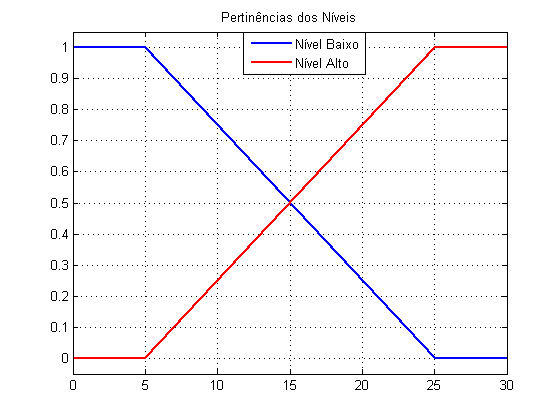
\includegraphics[width=0.7\textwidth]{img/pert_niveis.png}
	\caption{\label{figPertMod} Funções de Pertinência.}
\end{figure} 

Onde $M_1(h_1(t))$ e $M_2(h_1(t))$ é o grau de pertinência do nível $h_1(t)$ aos conjuntos "baixo" e "alto", respectivamente. De maneira análoga, tem-se $N_1(h_2(t))$ e $N_2(h_2(t))$ para o nível $h_2(t)$.

\subsection{Regras Se-Então}
Haverá uma regra para cada um dos sistemas dados:

	\begin{itemize}
		\item Regra 1:\\ 
		\begin{align*}
			\begin{cases}
				\text{SE } &h_1 \text{ é baixo e } h_2 \text{ é baixo} \\
				\text{ENTÃO } &\Delta \dot{h}(t) =  A_1 \Delta h(t) +  B_1 \Delta u(t)
			\end{cases}		
		\end{align*}

		\item Regra 2:\\ 
		\begin{align*}
		\begin{cases}
			\text{SE } &h_1 \text{ é baixo e } h_2 \text{ é alto} \\
			\text{ENTÃO } &\Delta \dot{h}(t) =  A_2 \Delta h(t) +  B_2 \Delta u(t)
		\end{cases}		
		\end{align*}

		\item Regra 3:\\ 
		\begin{align*}
		\begin{cases}
			\text{SE } &h_1 \text{ é alto e } h_2 \text{ é baixo} \\
			\text{ENTÃO } &\Delta \dot{h}(t) =  A_3 \Delta h(t) +  B_3 \Delta u(t)
		\end{cases}		
		\end{align*}

		\item Regra 4:\\ 
		\begin{align*}
		\begin{cases}
			\text{SE } &h_1 \text{ é alto e } h_2 \text{ é alto} \\
			\text{ENTÃO } &\Delta \dot{h}(t) =  A_4 \Delta h(t) +  B_4 \Delta u(t)
		\end{cases}		
		\end{align*}
	\end{itemize}

\subsection{Ativação}
O nível de ativação de cada uma das \textbf{Regras} $i$ é dado respectivamente por $w_i$:
	\begin{equation}
	\begin{aligned}
		w_{1}(t) = M_1(h_1(t)) * N_1(h_2(t)) \\
		w_{2}(t) = M_1(h_1(t)) * N_2(h_2(t)) \\
		w_{3}(t) = M_2(h_1(t)) * N_1(h_2(t)) \\
		w_{4}(t) = M_2(h_1(t)) * N_2(h_2(t))
	\end{aligned}
	\label{eqGrauAtiv4T}
	\end{equation}
	
\subsection{Modelo Final}
O peso de cada regra, na ponderação final, é dado por:
\begin{equation*}
	\alpha_i (h(t)) := \frac{w_i(h(t))}{\sum_{j=1}^{r}w_j(h(t))}
\end{equation*}

O modelo Takagi-Sugeno fornece, finalmente:
	\begin{align} \label{eqTakSugPlanta}
		\Delta \dot{h}(t) = \sum_{i=1}^{4} \alpha_i (h(t))(A_i \Delta h(t) +  B_i \Delta u(t))
	\end{align}


\subsection{Controlador Fuzzy}
No \jhhref{capControle}{Capítulo} demonstra-se o projeto de controladores capazes de estabilizar o sistema em todos os pontos de \ref{eqTakSugPlanta}. O desenvolvimento do controlador final para modelo segue os mesmos passos já apresentados: realiza-se a sintonização do ganho $K$ a ser utilizado para cada regra e o grau de ativação de cada ganho é obtido pelas mesmas \jhhref{eqGrauAtiv4T}{Equações}.
 O ganho final a ser utilizado é dado por:
	\begin{align*}
		K = \frac{\sum_{i=1}^{4}  w_i(h(t))K_i}{\sum_{i=1}^{4} w_i(h(t))}
	\end{align*}
	
Ou seja,

\begin{align} \label{eqModContFuzzy}
K = \sum_{i=1}^{4}  \alpha_i (h(t)) K_i
\end{align}

Deseja-se neste trabalho obter um controlador capaz de prover erro nulo para ambas os níveis inferiores em estado estacionário. Desta forma, foi desenvolvido um projeto aumentado dos erros integrais das variáveis controlados. O modelo final dos sistema é apresentado na \jhhref{figSimPlantCtrl}{Figura} a seguir:

\begin{figure}[H]
	\begin{centering}
		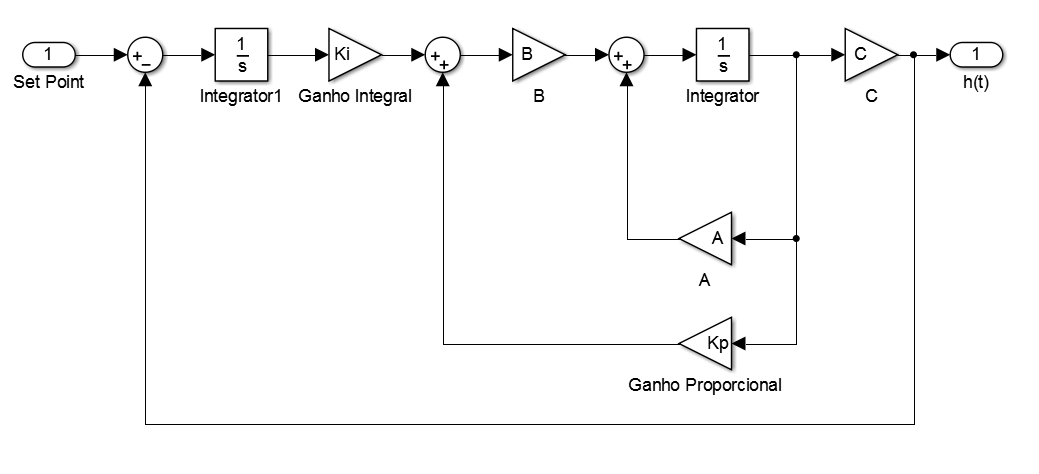
\includegraphics[width=\textwidth]{img/modelo_controlado.png}
		\par\end{centering}
	\caption{\label{figSimPlantCtrl}Espaço de estados da planta controlada}
\end{figure}

\selectlanguage{brazil}%

